\documentclass{article}
\usepackage{listings}  % Required for code formatting
\usepackage{xcolor}    % For color support
\usepackage{graphicx}
\usepackage{geometry}
\geometry{top=2cm, left=2cm, right=2cm, bottom=2cm}


% Custom settings for the listings package
\lstset{ 
  language=Python,               % Set the language to Python
  backgroundcolor=\color{white}, % Set background color for the code block
  basicstyle=\ttfamily\footnotesize,  % Use a typewriter font, and smaller size
  keywordstyle=\color{blue},     % Color for keywords (e.g. def, if, for)
  commentstyle=\color{green},    % Color for comments
  stringstyle=\color{red},       % Color for strings
  showstringspaces=false,        % Don't underline spaces in strings
  numberstyle=\tiny\color{gray}, % Style of line numbers
  numbers=left,                 % Position of line numbers
  stepnumber=1,                 % Show line numbers for every line
  numbersep=5pt,                % Distance between line numbers and code
  tabsize=4,                    % Set tab size
  captionpos=b,                 % Position of the caption (bottom)
  breaklines=true,              % Automatically break long lines
  breakatwhitespace=true,       % Break lines only at whitespace
  showtabs=false,                % Don't show tabs
  showspaces=false,              % Don't show spaces
  showstringspaces=false        % Don't show string spaces
}

\begin{document}

\title{Leavitt Law Calibration Python Library}
\author{Shubham Mamgain}
\date{\today}

\maketitle

%\tableofcontents
\section{Calibration}

\begin{figure}[h!]
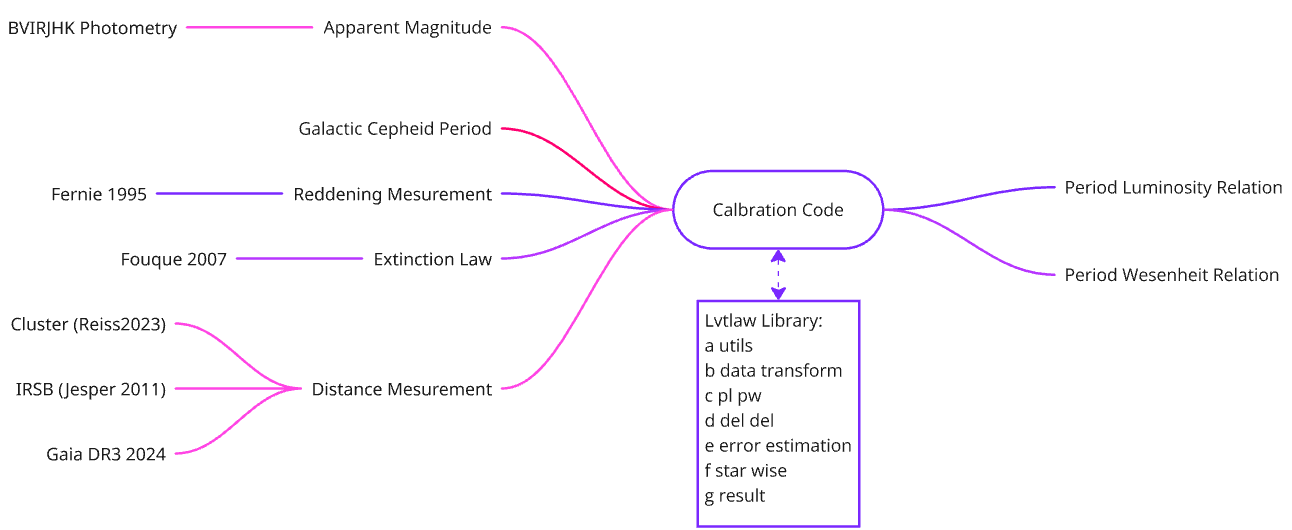
\includegraphics[width=\textwidth]{./figures/calibration.png}
\end{figure}


The calibration code executed by main.py file. The file is stored in parent directory of \textit{lvtlaw} library. Upon execution, it calls different modules of the library. Following is the description of each of the seven modules of the library.
\begin{lstlisting}[language=Python]
# main.py calls following modules
from lvtlaw.a_utils import load_data, input_data_file...
from lvtlaw.b_data_transform import transformation, extinction_law
from lvtlaw.c_pl_pw import pl_reg     
from lvtlaw.d_del_del import residue_analysis
from lvtlaw.e_error_estimation import reddening_error...
from lvtlaw.f_star_wise import star_frame, star_ex_red_mu
from lvtlaw.g_result import correction_rd_mu, correction_apply
raw_data = load_data(input_data_file)
\end{lstlisting}


\newpage
\subsection{lvtlaw.a\_utils}


\begin{figure}[h!]
\caption{\small datafile metadata mapping, mathematical tools definition, wesenheit color index}
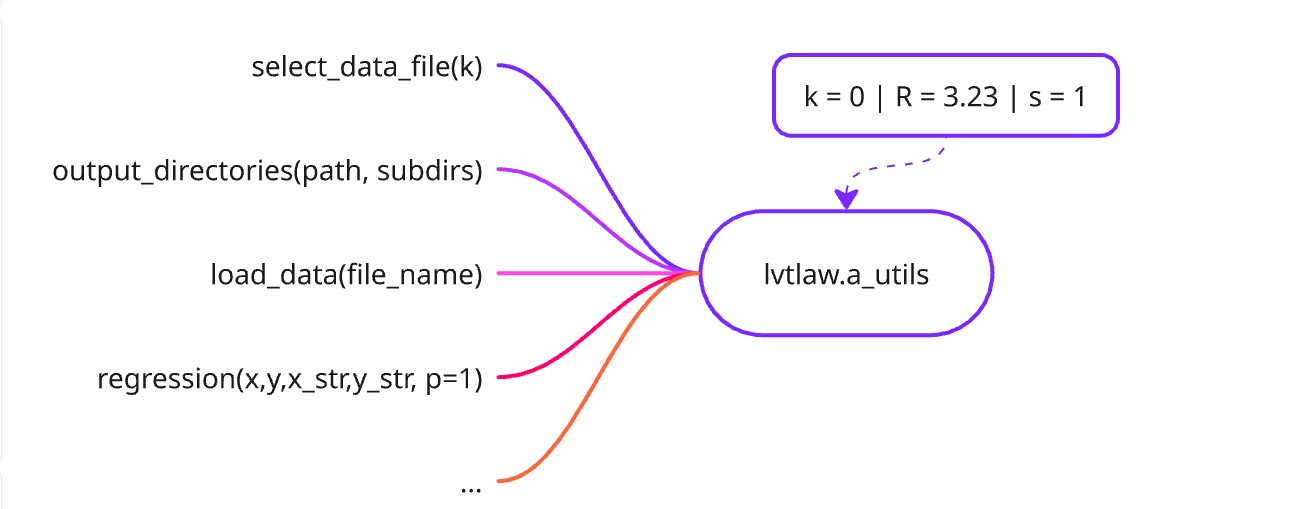
\includegraphics[width=\textwidth]{./figures/a_utils.png}
\end{figure}



\begin{lstlisting}[language=Python, caption=edit this function as per input dataset]
k = 2; # [0 ,1, 2 = Madore, Jesper, Reiss]

def select_data_file(k):
    if k==0:
        file_name = '59_madore.csv'
        file_cols = ['name','logP','HST','EBV','M_B','M_V'...] 
        dis_list = ['HST']
        R = [R_b, R_v, R_r, R_i, R_j, R_h, R_k]
        mag = ['B', 'V', 'R', 'I','J','H','K'];
    elif k ==1:
        file_name = '94_jesper.csv'
        file_cols = ['name',"logP", 'plx','IRSB', 'EBV', "B_mag", 'V_mag',...]
        dis_list = ['plx', 'IRSB']
        R = [R_b, R_v, R_i, R_j, R_h, R_k]
        mag = ['B', 'V', 'I','J','H','K'];
    elif k == 2:
        file_name = '18_gaia_irsb_cluster.csv'
        file_cols = ['name',"logP", 'cluster', 'EBV', "B_mag", 'V_mag'...]
        dis_list = ['cluster']
        R = [R_b, R_v, R_i, R_j, R_h, R_k]
        mag = ['B', 'V', 'I','J','H','K'];
    return file_name, file_cols, dis_list, R, mag

\end{lstlisting}

The file a\_utils.py provides data-related details to main.py via parameter k. The function select\_data\_file(k) maps the metadata of input file with data pipeline defined variables. The file also contains input/output related variables and some generic function like regression, save\_data, etc..


\newpage
\subsection{lvtlaw.b\_data\_transform}

\begin{figure}[h!]
\caption{\small datafile metadata mapping, mathematical tools definition, wesenheit color index}
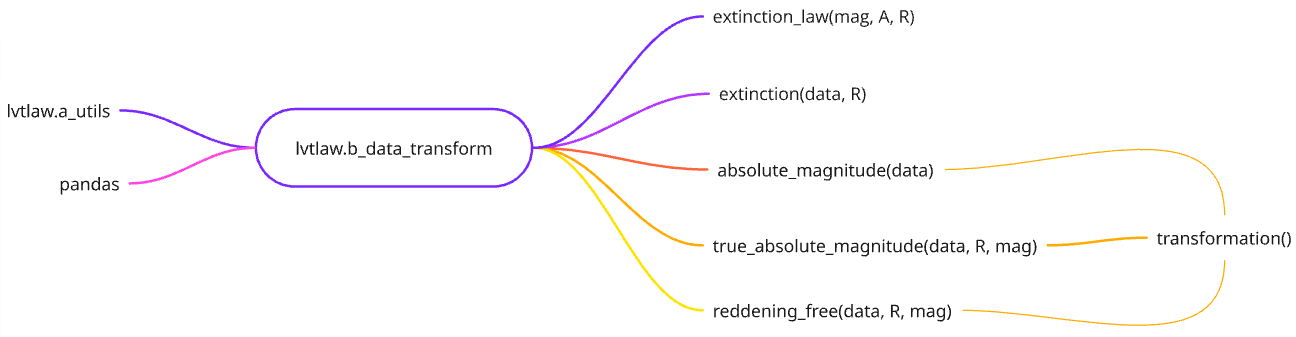
\includegraphics[width=\textwidth]{./figures/b_data_transform.png}
\end{figure}



\begin{lstlisting}[language=Python, caption=edit this function as per input dataset]
def reddening_free(data, R=R, mag=mag, ap_bands=ap_bands):
    wesen = pd.DataFrame()
    wesen['logP'] = data['logP']
    for a in range(0,len(mag)):
        for b in range(a+1,len(mag)):
            for c in range(0,len(mag)):
                for d in range(0,len(dis_list)):
                    wes_str = mag[c]+mag[a]+mag[b]+dis_flag[d]
                    if k == 0: # Madore
                        wesen[wes_str] = data[abs_bands[c]] - (R[c]/(R[a]-R[b]))*(data[abs_bands[a]] - data[abs_bands[b]])
                    elif k==1: # Jesper
                        wesen[wes_str] = data[ap_bands[c]] - (R[c]/(R[a]-R[b]))*(data[ap_bands[a]] - data[ap_bands[b]]) - data[dis_list[d]]
                    elif k==2: # Riess
                        wesen[wes_str] = data[ap_bands[c]] - (R[c]/(R[a]-R[b]))*(data[ap_bands[a]] - data[ap_bands[b]]) - data[dis_list[d]]
    return wesen

def transformation(data):
    print('Absolute magnitude for each band \n')
    abs_data = absolute_magnitude(data)    
    print('Calculated extinction for each band \n')
    ext_data = extinction(data)
    print('True absolute magnitude for each band \n')
    tabs_data = true_absolute_magnitude(data)
    print('Wesenheit magnitude for each band \n')
    wes_data = reddening_free(data)
    return  abs_data, ext_data, tabs_data, wes_data
        
\end{lstlisting}



'b\_data\_transform.py' converts raw data into absolute magnitude, true absolute magnitude, wesenheit magnitude and save the tables in output/1\_prepared directory. Another function provides Fouque extinction law to convert reddening into extinction. 

\newpage
\begin{figure}[h!]
\caption{\small datafile metadata mapping, mathematical tools definition, wesenheit color index}
\includegraphics[width=\textwidth]{./data/output/9_plots/2_PLPW/59_PL_B_h.png}
\includegraphics[width=\textwidth]{./data/output/9_plots/2_PLPW/59_PL_V_h.png}
%\includegraphics[width=\textwidth]{./data/output/9_plots/2_PLPW/59_PL_R_h.png}
\includegraphics[width=\textwidth]{./data/output/9_plots/2_PLPW/59_PL_I_h.png}
\includegraphics[width=\textwidth]{./data/output/9_plots/2_PLPW/59_PL_J_h.png}
\includegraphics[width=\textwidth]{./data/output/9_plots/2_PLPW/59_PL_H_h.png}
\includegraphics[width=\textwidth]{./data/output/9_plots/2_PLPW/59_PL_K_h.png}
\end{figure}



\newpage
\subsection{lvtlaw.c\_pl\_pw}
\begin{figure}[h!]
\caption{\small datafile metadata mapping, mathematical tools definition, wesenheit color index}
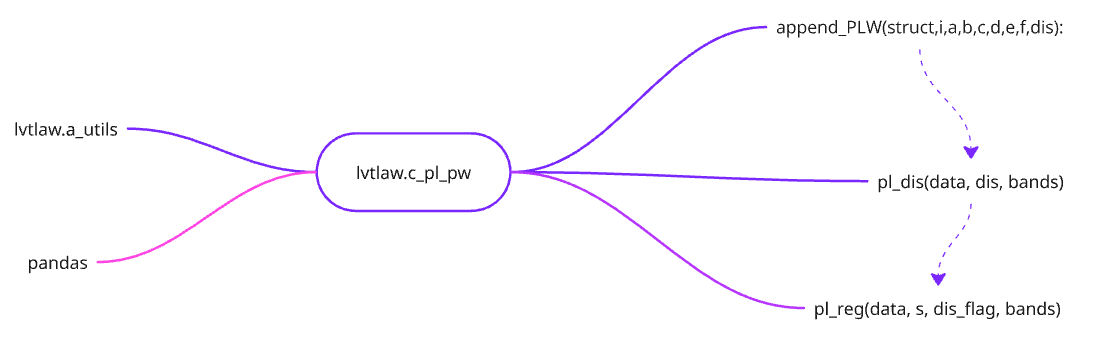
\includegraphics[width=\textwidth]{./figures/c_pl_pw.png}
\end{figure}


\begin{lstlisting}[language=Python, caption=dependencies for main.py]
def pl_dis(data, dis: str, mag: list):
    PL_name, PL_slope, PL_intercept = [], [], []
    err_slope, err_intercept = [], []
    residue = pd.DataFrame({'name': data['name'], 'logP': data['logP']})
    prediction = residue.copy()   
    # Store regression results
    PLW_struct = [PL_name, PL_slope, PL_intercept, prediction, residue, err_slope, err_intercept]    
    for i in range(len(mag)):  # Absolute Magnitude
        a, b, c, d, e, f = regression(data['logP'] - 1, data[bands[i] + dis], '(logP - 1)', bands[i] + dis, 1)
        PLW_struct = append_PLW(PLW_struct, mag[i], a, b, c, d, e, f, dis)
    for i in range(len(mag)):  # True absolute magnitudes
        a, b, c, d, e, f = regression(data['logP'] - 1, data[bands[i] + '0' + dis], '(logP -1)', bands[i] + '0' + dis, 1)
        PLW_struct = append_PLW(PLW_struct, mag[i] + '0', a, b, c, d, e, f, dis)
    for color in wes_show: #Wesenheit Magnitude for color index
        for i in range(len(mag)):
            a, b, c, d, e, f = regression(data['logP'] - 1, data[mag[i] + color + dis], '(logP - 1)', mag[i] + color + dis, 1)
            PLW_struct = append_PLW(PLW_struct, mag[i] + color, a, b, c, d, e, f, dis)
    
    # Convert the results into a DataFrame
    PLW = pd.DataFrame({
        'name': PLW_struct[0],
        f'm{dis}': PLW_struct[1],
        f'c{dis}': PLW_struct[2],
        f'err_m{dis}': PLW_struct[5],
        f'err_c{dis}': PLW_struct[6]
    })
    prediction = PLW_struct[3]
    residue = PLW_struct[4]
    
    return PLW, residue, prediction

def pl_reg(data, dis_flag: list):
    reg = pd.DataFrame()
    res = pd.DataFrame()
    pre = pd.DataFrame()
    for dis in dis_flag:
        PLW, residue, prediction = pl_dis(data, dis, bands)
        reg = pd.concat([reg, PLW], axis=1)
        res = pd.concat([res, residue], axis=1)
        pre = pd.concat([pre, prediction], axis=1)
    return reg, res, pre

\end{lstlisting}



'c\_pl\_pw.py' deduces the PL and PW relations from prepared data and save their residues, prediction and slope\_intercept data in output/2\_PLPW directory.


\newpage
\subsection{lvtlaw.d\_del\_del}
\begin{figure}[h!]
\caption{\small datafile metadata mapping, mathematical tools definition, wesenheit color index}
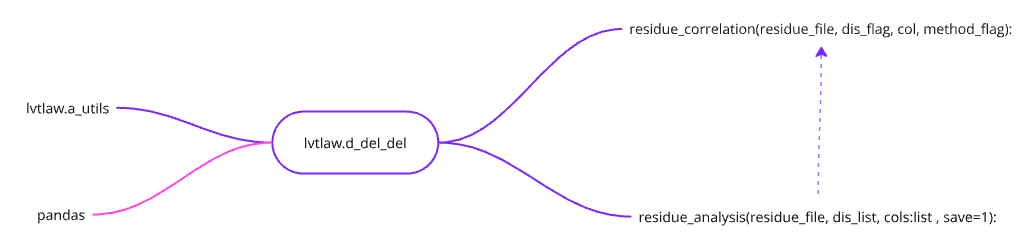
\includegraphics[width=\textwidth]{./figures/d_del_del.png}
\end{figure}


\begin{lstlisting}[language=Python, caption=dependencies for main.py]
def residue_correlation(residue_file, dis_flag, col, method_flag):
    ...
    for diss in dis_flag:
        for band in mag:
            wesenheit = f"{band}{col}" 
            x_key = 'r_' + wesenheit + diss
            y_key = 'r_' + band + '0' + diss
            # Perform regression
            slope, intercept, predicted, residual, slope_err, intercept_err = regression(
                residue_file[x_key], residue_file[y_key], wesenheit, band + '0' + diss, 1)
            ...
        # Save regression metadata for this distance flag
        del_mc[f'm{diss}'] = slopes
        ...
    return del_residuals, del_predictions, del_mc

def residue_analysis(residue_file, dis:list, cols:list , save=1):
    ...
    for col in cols:
        res, pre, mc = residue_correlation(residue_file, dis, col)
        dres = pd.merge(dres, res, on='name')
        dpre = pd.merge(dpre, pre, on='name')
        dmc.append(mc)
    # Combine regression dataframes
    dmc = pd.concat(dmc, ignore_index=True).drop_duplicates().set_index('name').T
    dSM = [[dmc_S],[dres_S]]
    return dres_S, dpre_S, dres_M, dpre_M, dSM

\end{lstlisting}

'd\_del\_del.py' contains two functions: a) residue\_analysis which retrieves PL-PLW residue for correlation according to Madore and Shubham approach as two separate cases. b) residue\_correlation - correlates given PL PW residues for each band. Slope, intercept, residue are saved at output/3\_deldel directory.


\newpage
\subsection{lvtlaw.e\_error\_estimation}

\begin{figure}[h!]
\caption{\small datafile metadata mapping, mathematical tools definition, wesenheit color index}
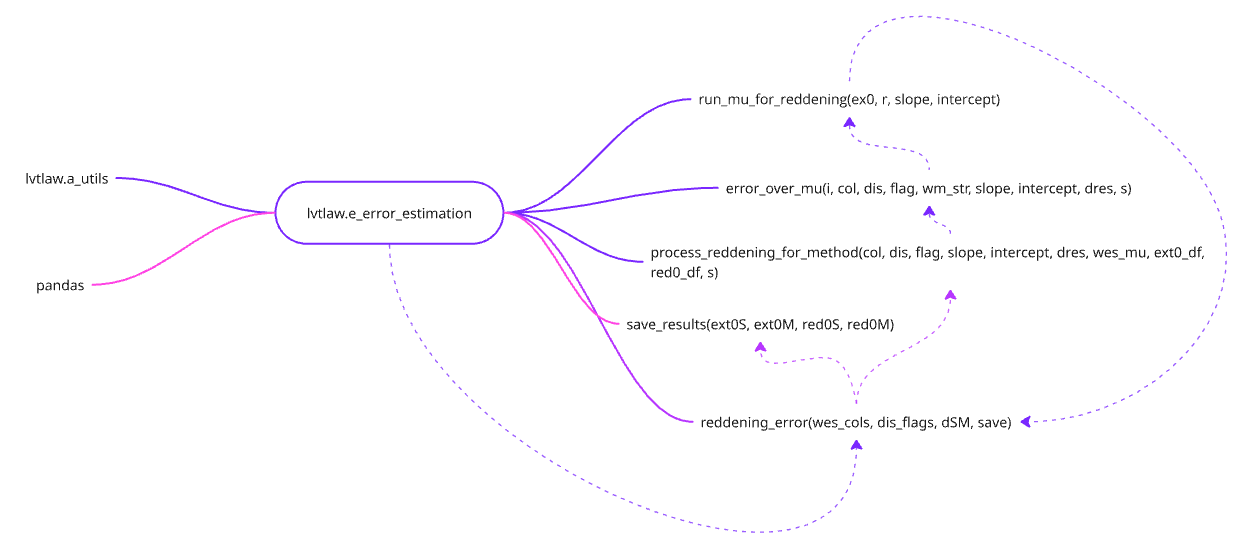
\includegraphics[width=\textwidth]{./figures/e_error_estimation.png}
\end{figure}

\begin{lstlisting}[language=Python, caption=dependencies for main.py]
def run_mu_for_reddening(ex0, r, slope, intercept):
    # for given star, estimate reddening for different mu
    mu_run = pd.DataFrame() 
    for mu in del_mu:
        mu_run[f'ex_{mu}'] = ex0 + mu * (1 - slope) - intercept
        mu_run[f'rd_{mu}'] = mu_run[f'ex_{mu}'] / r
    return mu_run

def error_over_mu(i, col, dis, flag, wm_str, slope, intercept, dres, s):
    r = R[i] / (R[0] - R[1])  # reddening ratio B-V
    slope = slope[wm_str]
    intercept = intercept[wm_str]
    ext0 = dres[f'd_{wm_str}{dis}']
    red0 = ext0 / r  # Convert extinction to reddening E(B-V)
    mu_run_ext_red = run_mu_for_reddening(ext0, r, slope, intercept)
    return ext0, red0, mu_run_ext_red

def process_reddening_for_method(col, dis, flag, slope, intercept, dres, wes_mu, ext0_df, red0_df, s):
    for i, band in enumerate(mag):
        wm_str = f"{band}{col[0]}{col}" if flag == '_M' else f"{band}{band}{col}"
        ext0, red0, mu_err = error_over_mu(i, col, dis, flag, wm_str, slope, intercept, dres, s)        
        ext0_df[f'{wm_str}{dis}'] = ext0
        red0_df[f'{wm_str}{dis}'] = red0
        wes_mu.append(mu_err)
    return wes_mu

def reddening_error(wes_cols, dis_flags, dSM, save=1):
    ...
    for dis in dis_flags:
        m_S, c_S, m_M, c_M = select_regression_parameters(dSM, dis)
        dis_mu_dict = {}
        for col in wes_cols:
            wes_mu_S, wes_mu_M = [], []
            # Madore approach
            wes_mu_M = process_reddening_for_method(col, dis, '_M', m_M, c_M, dSM[1][1], wes_mu_M, ext0M, red0M, save)       
            # Shubham approach
            wes_mu_S = process_reddening_for_method(col, dis, '_S', m_S, c_S, dSM[1][0], wes_mu_S, ext0S, red0S, save)
            dis_mu_dict[f'{col}_M'] = wes_mu_M
            dis_mu_dict[f'{col}_S'] = wes_mu_S
        ex_rd_mu.append(dis_mu_dict)
    red_SM = [red0S, red0M]
    save_results(ext0S, ext0M, red0S, red0M)
    return red_SM, ex_rd_mu


\end{lstlisting}

'e\_error\_estimation.py' has four functions. a) reddening\_error() retrieves input using select\_regression\_parameters() and feed output to process\_reddening\_for\_method() for both approaches separately. It yields extinction-reddening error-matrix contain all stars. b) process\_reddening\_for\_method calls error\_over\_mu() which extrapolates reddening error for different modulus error and save result for each wesenheit case.  


\newpage
\subsection{lvtlaw.f\_star\_wise}

\begin{figure}[h!]
\caption{\small datafile metadata mapping, mathematical tools definition, wesenheit color index}
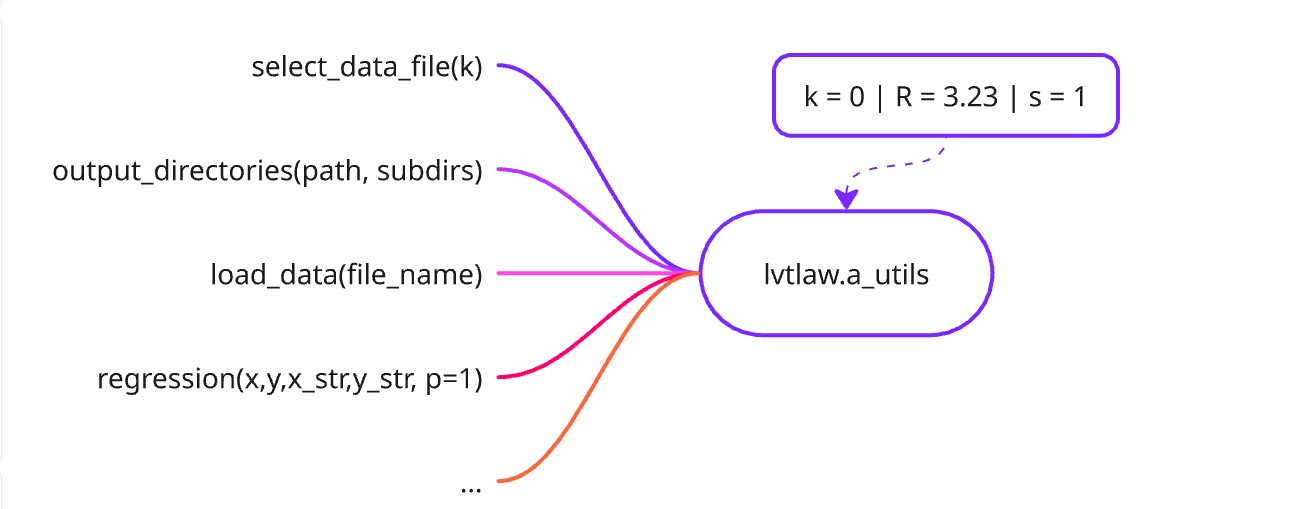
\includegraphics[width=\textwidth]{./figures/f_star_wise.png}
\end{figure}

\begin{lstlisting}[language=Python, caption=dependencies for main.py]
def star_ex_red_mu(n, ex_rd_mu, raw):
    stars = []
    print('Reddenings over mu for each star, each color and respective distance')
    for i in range(0, n):
        df = pd.DataFrame()
        for d in range(len(dis_flag)):
            for c in wes_show:
                rdS = pd.DataFrame()
                rdM = pd.DataFrame()
                for m in range(len(mag)):
                    rdS[mag[m]] = ex_rd_mu[d][c+'_S'][m][['rd_'+str(mu) for mu in del_mu]].iloc[i].values
                    rdM[mag[m]] = ex_rd_mu[d][c+'_M'][m][['rd_'+str(mu) for mu in del_mu]].iloc[i].values
                rdS = rdS.T
                rdS.columns = [[c+dis_flag[d]+'rd_S'+strtmu) for mu in del_mu]]  # Make sure number matches df.shape[1]
                rdM = rdM.T
                rdM.columns = [[c+dis_flag[d]+'rd_M'+str(mu) for mu in del_mu]]  # Make sure number matches df.shape[1]
                df = pd.concat([df, rdM], axis=1)                         
                df = pd.concat([df, rdS], axis=1)   
                df.loc['mean'] = df.mean()
                df.loc['var'] = df.var()                       
            print('#'*30)
        #print(df)
        stars.append(df)
        print('Star Name: ', raw.name.iloc[i])
        print(i, stars[i])                         
        df.to_csv('%s%i_%istars_ex_red_mu.csv'%(data_out+process_step[5],i, n))
    return stars
            
\end{lstlisting}

f\_star\_wise.py extract error-matrix for each star containing all wesenheit cases in a single table. It also collects reddening error-matrix for different modulus



\newpage
\subsection{lvtlaw.g\_result}
\begin{figure}[h!]
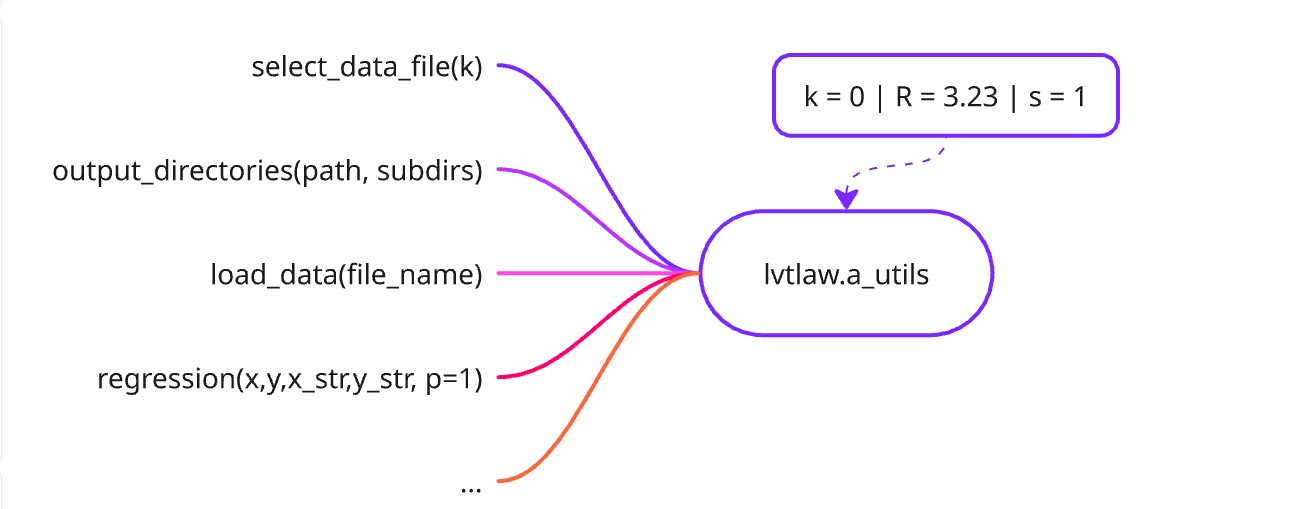
\includegraphics[width=\textwidth]{./figures/g_result.png}
\caption{\small datafile metadata mapping, mathematical tools definition, wesenheit color index}
\end{figure}

\begin{lstlisting}[language=Python, caption=dependencies for main.py]
def get_error_pair(star):
    ls = {}    # 
    for d in dis_flag:
        for col in wes_show: 
            for f in flags:
                x = star[[col+d+'rd'+f+str(mu) for mu in del_mu]].iloc[-1]# # variance list
                x_min = pd.to_numeric(x, errors='coerce').min()   # minimum variance
                mu_name = star[[col+d+'rd'+f+str(mu) for mu in del_mu]].iloc[-1].idxmin()  # collect mu index
                rd = star[mu_name[0]].iloc[-2]  # collect mean reddening 
                mu = float(mu_name[0][8:])  # collect mu
                ls['rms'+d+col+f] = x_min 
                ls['mu'+d+col+f] = mu
                ls['rd'+d+col+f] = rd.iloc[0]#.values 
    return ls

def correction_rd_mu(stars, save=1):
    stars_correction = [] 
    for i in range(len(stars)):
        mu_rd_pair_list = get_error_pair(stars[i])
        stars_correction.append(mu_rd_pair_list)
    correction_red_mu_stars = pd.DataFrame(stars_correction)
    if save==1:
        correction_red_mu_stars.to_csv('%s%i_error_rms_mu_rd.csv'%(data_out+process_step[6],len(stars)))
    return correction_red_mu_stars    

def correction_apply(tabsolute, correction, save=1):
    corrected = pd.DataFrame()
    correct = pd.DataFrame()
    corrected['logP'] = tabsolute['logP'] 
    for d in dis_flag:
        for col in wes_show:
            for f in flags:
                correct['mu'+d+col+f] = correction['mu'+d+col+f]
                for i in range(len(mag)):
                    correct['ex'+mag[i]+d+col+f] = R[i]*correction['rd'+d+col+f]
                    corrected[mag[i]+d+col+f]=tabsolute['M_'+mag[i]+'0'+d] + correct['ex'+mag[i]+d+col+f]+correction['mu'+d+col+f]
    print('Correction for each band \n', correct)
    if save==1:
        corrected.to_csv('%s%i_corrected_%s%s%s.csv'%(data_out+process_step[7],len(corrected), d, col, f))
    return corrected
    
def corrected_PL(tabsolute, corrected, s=1):
    for dis in dis_flag:
        for col in wes_show:
            for flag in flags:
                print('Method: ', flag[1], '\t Color: ', col, '\t Distance: ', dis[1])
                for i in range(len(mag)):
                    regression(tabsolute['logP']-1, tabsolute['M_'+mag[i]+'0'+dis], '(logP - 1)', 'M__'+mag[i], 1)
                    m,c,p,r,em,ec = regression(corrected['logP']-1,corrected[mag[i]+dis+col+flag], '(logP - 1)', 'M*_%s'%(mag[i]), p = s)
    #if save==1:
        #corrected.to_csv('%s%i_corrected_%s%s%s.csv'%(data_out+process_step[6],len(corrected),col, dis, flag))
        
        
\end{lstlisting}

g\_result.py has four functions. a) get\_error\_pair retrives the distance-reddening error pair for each star for each wesenheit case, and both approaches. b) correction\_rd\_mu collects the correction for each stars, for both approaches and all weseheit cases, and returns a correction-pair table. c) correction\_apply impliments the correction on the input data. d) corrected\_PL() generates the new PL relations. 


\end{document}



